\chapter{An simple example of chapter title with a very large length}

\begin{phrasebox}{}{\textit{The author name}}
\label{phrasebox:2}
\textit{\lipsum[1][1-3]}
\end{phrasebox}

\vspace{1ex}
\lipsum[1][1-4] 
%-------------------------------------------------------------------------------
\section{A simple example of section title with a very large length}\index{Paragraphs of Text}

\lipsum[1][1-3] 
Referencia a la Información \ref{informationbox:1} (siguiente)

\begin{informationbox}[Título A]
\label{informationbox:1}
\lipsum[1][1-3] 
\end{informationbox}

\lipsum[1]

\SeparatorTextRule{A very very large text in a separator rule}%{Text}%
\lipsum[1][1-3]
Referencia a las Frases \ref{phrasebox:1} y \ref{phrasebox:2} 

\begin{phrasebox}{Frase title A}{Autor}
\label{phrasebox:1}
\lipsum[1][1-2] 
\end{phrasebox}

\lipsum[1][1-3] 

\begin{citationbox}
\lipsum[1][1-3] 
\end{citationbox}

%-------------------------------------------------------------------------------
\section{Another title}\index{Index B}

This statement requires citation \cite{book_key}; this one is more specific \cite[122]{article_key}.
\lipsum[1][1-4]
 
Referencia a la Información \ref{information:2} (siguiente)

\begin{informationbox}[Título B]
\label{information:2}
\lipsum[1][1-3]\footnote{Simple footnote example.}
\end{informationbox}

\lipsum[1] % 

\begin{attentionbox}
\label{attentionbox:a}
\lipsum[1][1-3]\footnote{Simple footnote example.}
\end{attentionbox}

\lipsum[1] % 

Referencia a la Información \ref{elaboration:3} (siguiente)

\begin{elaboration}[Título C]
\label{elaboration:3}
\lipsum[1][1-3] 
\end{elaboration}

\lipsum[1][1-3] %


Referencia a la Notacion \ref{notation:0} (siguiente)

\begin{notation}[Título C]
\label{notation:0}
\lipsum[1][1-2]
\begin{itemize}
\item \lipsum[1][1-2]
\item \lipsum[1][1-2]
\begin{itemize}
\item \lipsum[1][1-2]
\item \lipsum[1][1-2]
\end{itemize}
\end{itemize}
\end{notation}

\lipsum[1][1-3] %

Referencia a la Notacion \ref{notation:1} (siguiente)

\begin{notation}[Título C]
\label{notation:1}
\lipsum[1][1-2]
\begin{enumerate}
\item \lipsum[1][1-2]
\item \lipsum[1][1-2]
\begin{enumerate}
\item \lipsum[1][1-2]
\item \lipsum[1][1-2]
\end{enumerate}
\end{enumerate}
\end{notation}

%-------------------------------------------------------------------------------
\section{Another simple title example with a very large length}
\index{Theorem  family}

\lipsum[1][1-3].
\begin{enumerate}
\item \lipsum[1][1-2]
\item \lipsum[1][1-2]
\begin{enumerate}
\item \lipsum[1][1-2]
\item \lipsum[1][1-2]
\end{enumerate}
\end{enumerate}
\lipsum[1][1-3]. See the Theorem \ref{theo:ex1:A} and Figure \ref{fig:exemplo}.
The Figure was generated by \CommandBox{chapters/cap1/python/example.py}.

\begin{figure}[htbp] % 'htbp' é uma sugestão de posicionamento
  \centering          % Centraliza a figura
  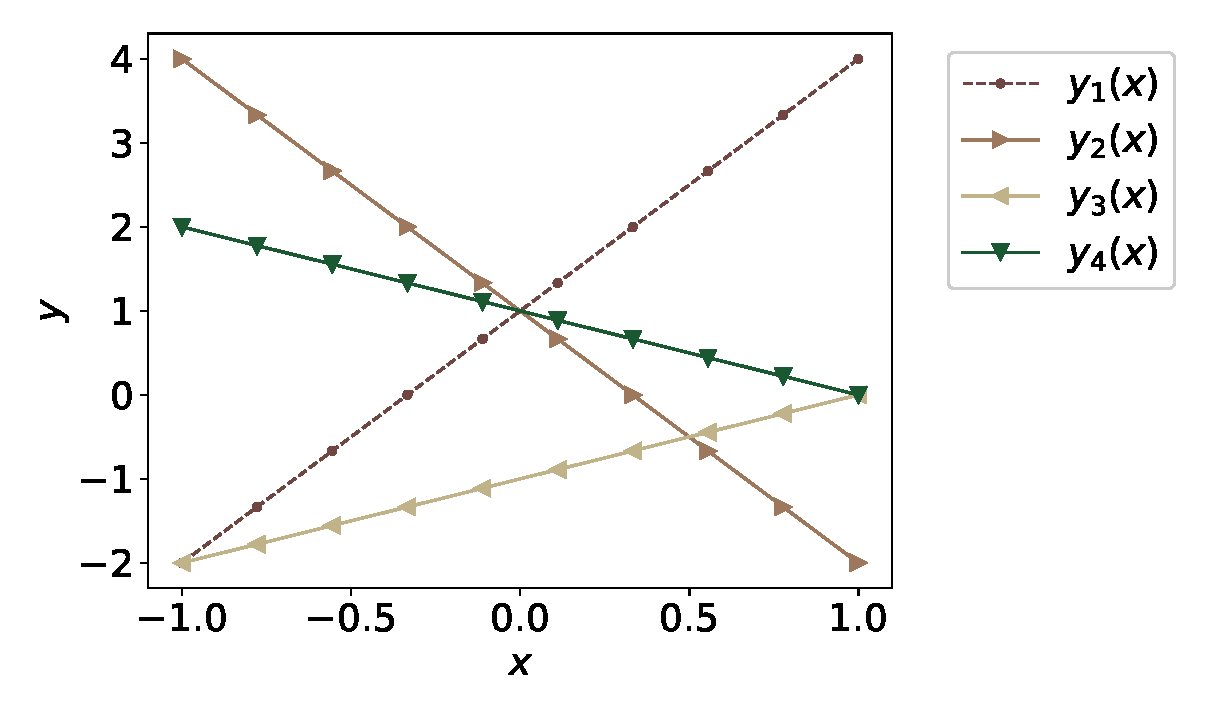
\includegraphics[width=0.75\textwidth]{chapters/cap1/python/example.eps}
  \caption{Image with the same color scheme of book} % Adiciona uma legenda
  \label{fig:exemplo} % Adiciona um rótulo para referência
\end{figure}


\begin{theorem}[Name of the theorem]
\label{theo:ex1:A}
\lipsum[1][1-3]
\begin{equation}
x^2+e^{-\frac{x^2}{2}}=1
\end{equation}
\end{theorem}

teste

\begin{proofraw}[Relative to Teorema \ref{theo:ex1:A}]
\lipsum[1][1-3]
\begin{equation}
x^2+e^{-\frac{x^2}{2}}=1
\end{equation}
\end{proofraw}
%-------------------------------------------------------------------------------
\section{Lists}\index{Lists}

\lipsum[1][1-3]\footnote{Footnote example...}.

\subsection{Numbered List}\index{Lists!Numbered List}

\begin{enumerate}
\item \lipsum[1][1-3].
\item \lipsum[1][1-3].
\item \lipsum[1][1-3].
\end{enumerate}

\subsection{Bullet Points}\index{Lists!Bullet Points}

\begin{itemize}
\item \lipsum[1][1-3].
\item \lipsum[1][1-3].
\item \lipsum[1][1-3].
\end{itemize}

\subsection{Descriptions and Definitions}\index{Lists!Descriptions and Definitions}

\begin{description}
\item[Name] \lipsum[1][1-3].
\item[Word] \lipsum[1][1-3].
\item[Comment] \lipsum[1][1-3].
\end{description}

